\chapter{Methodology}\label{chap4}

\section{High-Level View: System Architecture}

Figure~\ref{fig:architecture} presents a high-level view of the
proposed system architecture, which is fully based on the FIWARE
framework and NGSI-LD standard. The architecture follows a modular
design to enable real-time context management, historical data storage,
and visualization of electric vehicle (EV) charging infrastructure.

\begin{figure}[ht!]
    \centering
    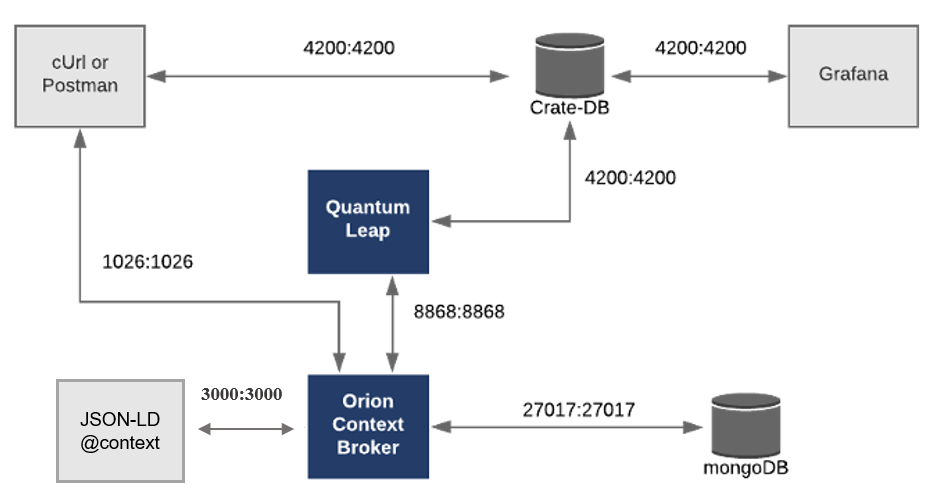
\includegraphics[width=0.7\textwidth]{Images/digiev-architecture.png}
    \caption{\textbf{DigiEV System Architecture}}
    \label{fig:architecture}
\end{figure}

At the core of the architecture lies the \textbf{Orion-LD Context Broker}
(port \texttt{1026}), which manages all NGSI-LD entities, properties,
and relationships. Incoming context data, described in JSON-LD, is
ingested into Orion through RESTful APIs (typically tested with cURL
or Postman). Orion ensures semantic interoperability by linking each
entity with its external \texttt{@context} definition, served by a JSON-LD
context server (port \texttt{3000}).

Two databases support the broker. \textbf{MongoDB} (port
\texttt{27017}) stores the latest state of entities and metadata, while
\textbf{CrateDB} (port \texttt{4200}) stores historical time-series data.
To bridge between Orion and CrateDB, the system employs
\textbf{Quantum Leap (QL)} (port \texttt{8868}), which subscribes to
Orion and translates every entity update into time-series entries stored
in CrateDB. In this way, QL decouples context management from
historical data persistence.

For visualization and monitoring, \textbf{Grafana} (also connected via
port \texttt{4200}) queries CrateDB directly, enabling the creation of
dashboards to analyze charging patterns, station utilization, and grid
impacts. This modular setup therefore provides both:
\begin{itemize}
  \item \emph{Real-time monitoring} of current states via Orion-LD and MongoDB.
  \item \emph{Historical analysis} via Quantum Leap, CrateDB, and Grafana.
\end{itemize}

\subsubsection*{Data Flow Description}

The workflow of the system can be summarized in the following steps:

\begin{enumerate}
  \item \textbf{Data ingestion:} Context information describing EV
  charging infrastructure (e.g., charging sessions, station status) is
  formatted in NGSI-LD (JSON-LD) and sent to the Orion-LD Context
  Broker (port \texttt{1026}) using REST APIs (via cURL or Postman).
  \item \textbf{Semantic enrichment:} Orion-LD validates the data against
  the JSON-LD \texttt{@context} (served on port \texttt{3000}), ensuring
  semantic consistency across entities, properties, and relationships.
  \item \textbf{Context storage:} Orion-LD stores the latest state of each
  entity in \textbf{MongoDB} (port \texttt{27017}), which acts as a
  short-term persistence layer for current context information.
  \item \textbf{Time-series processing:} The \textbf{QL}
  service (port \texttt{8868}) subscribes to Orion-LD. Every time Orion
  emits an update, QL converts it into a time-series entry and persists it
  in \textbf{CrateDB} (port \texttt{4200}).
  \item \textbf{Visualization and analytics:} \textbf{Grafana} connects to
  CrateDB (via port \texttt{4200}) to generate dashboards for both
  historical and real-time analysis of charging infrastructure, enabling
  insights into charging demand, station utilization, and grid impacts.
\end{enumerate}

This pipeline ensures that both the \emph{current state} of EV charging
infrastructure (via Orion-LD and MongoDB) and its \emph{historical
evolution} (via Quantum Leap and CrateDB) are available for analysis,
providing a comprehensive digital twin representation.

All services in the proposed architecture are containerized and deployed
using \textbf{Docker} and \textbf{Docker Compose}. Each component
(Orion-LD, MongoDB, Quantum Leap, CrateDB, Grafana, JSON-LD
context server) runs as an isolated container, exposing its standard
ports as shown in Figure~\ref{fig:architecture}. The use of
Docker provides several advantages:
\begin{itemize}
  \item \emph{Portability:} the whole architecture can be reproduced on
  different machines with minimal configuration.
  \item \emph{Isolation:} each service is encapsulated in its own
  container, avoiding dependency conflicts.
  \item \emph{Scalability:} containers can be scaled (e.g., multiple
  instances of Orion-LD or CrateDB) to handle higher workloads.
  \item \emph{Maintainability:} the configuration of all services,
  including port mappings and volumes, is defined in a single
  \texttt{docker-compose.yml} file, making the setup reproducible and
  easy to extend.
\end{itemize}

This containerized setup ensures that the FIWARE-based digital twin
system can be rapidly deployed, tested, and extended in practical
scenarios such as the E4C campus testbed.

\section{Design Data Model}

\subsection*{\texttt{@context} File}
Within the NGSI-LD standard, the \texttt{@context} file represents the cornerstone of semantic data modeling. Its main purpose is to provide globally unique and machine-readable identifiers (URIs) for entities, properties, and relationships. In this way, when different systems exchange data, they can not only understand the structure but also interpret the meaning of the information consistently.

In this project, to describe the digital twin of the charging infrastructure, I designed a dedicated \texttt{@context} file. The beginning of this file is shown below:

\begin{minted}[bgcolor=codebg,fontsize=\small,frame=lines,linenos]{python}
    "@context": {
        "type": "@type",
        "id": "@id",
        "ngsi-ld": "https://uri.etsi.org/ngsi-ld/",
        "fiware": "https://uri.fiware.org/ns/data-models#",
        "schema": "https://schema.org/",
        "ChargingPoint": "fiware:ChargingPoint",
        "ChargingPointStatus": "fiware:ChargingPointStatus",
        "ChargingSession": "fiware:ChargingSession",
        "ChargingStation": "fiware:ChargingStation"}
\end{minted}

\begin{itemize}
        \item \texttt{"type"} and \texttt{"id"} define the fundamental structure of NGSI-LD entities (their type and identifier).
        \item \texttt{"ngsi-ld"}, \texttt{"fiware"} and \texttt{"schema"} point to the NGSI-LD standard, the FIWARE data model repository, and the \texttt{schema.org} vocabulary, respectively. These ensure reusability and standard compliance of the model.
        \item \texttt{"ChargingPoint"} is defined as \texttt{fiware:ChargingPoint}, representing an individual charging connector.
        \item \texttt{"ChargingPointStatus"} describes the operational status of a connector (e.g., available, occupied, reserved).
        \item \texttt{"ChargingSession"} corresponds to a charging event triggered by a user interacting with the infrastructure.
        \item \texttt{"ChargingStation"} represents a physical charging facility that may host multiple charging points.
\end{itemize}

After defining the \texttt{@context} file, the next step was to design the entities and their interconnections. 
Figure~\ref{fig:PropertyGraph} illustrates the main components of the data model used in the digital twin of the charging infrastructure. 

\subsection*{Static and Dynamic Entities}
The model is structured around a clear distinction between:
\begin{itemize}
    \item \textbf{Static entities:} These describe relatively stable infrastructure components such as \texttt{ChargingStation}, \texttt{ChargingPoint}, and \texttt{EV}. Their properties change rarely (e.g., location, maximum power).
    \item \textbf{Dynamic entities:} These represent operational states that evolve over time, such as \texttt{StationStatus}, \texttt{PointStatus}, \texttt{EVStatus}, and particularly the \texttt{ChargingSession}. Dynamic entities are the key carriers of time-series data.
\end{itemize}

\subsection*{Bidirectional Relationships}
The model also supports bidirectional relationships to ensure semantic consistency across the system. For example:
\begin{itemize}
    \item A \texttt{ChargingPoint} is linked to its parent \texttt{ChargingStation} through \texttt{refChargingPoint}, while the reverse relation \texttt{refChargingStation} allows navigation back from the station to its connectors.
    \item A \texttt{ChargingSession} is associated with both the \texttt{ChargingPoint} and the \texttt{EV}, reflecting the real-world interaction between the vehicle and the infrastructure. The reverse relations (\texttt{refChargingSession}) enable tracing sessions from either perspective.
\end{itemize}

\begin{figure}[ht!]
    \centering
    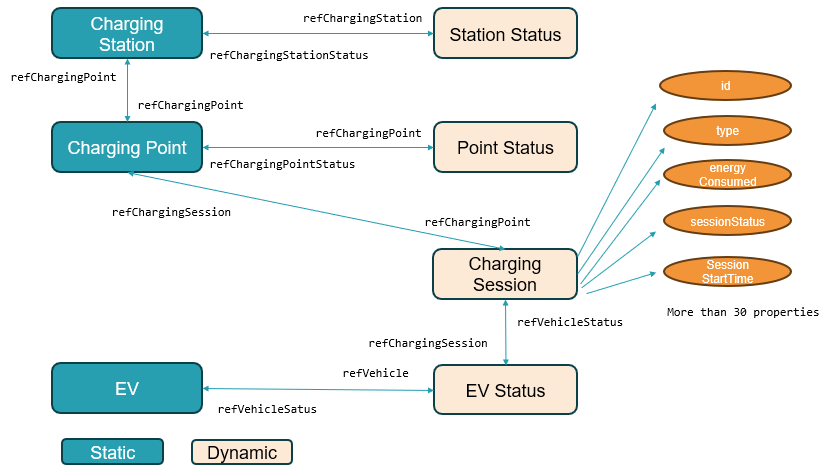
\includegraphics[width=0.7\textwidth]{Images/Property Graph.png}
    \caption{\textbf{Entity and relationship structure (Property Graph)}}
    \label{fig:PropertyGraph}
\end{figure}

\subsection*{Entity Properties}
Each entity contains a set of attributes. For example, a \texttt{ChargingSession} may include more than 30 properties, such as:
\begin{itemize}
    \item \texttt{id}, \texttt{type}: core NGSI-LD attributes.
    \item \texttt{sessionStartTime}: the timestamp when the session begins.
    \item \texttt{energyConsumed}: the amount of electricity delivered during the session.
    \item \texttt{sessionStatus}: operational status of the session (authorized, charging, completed etc\@.).
\end{itemize}

By structuring the model in this way, the digital twin can accurately represent both the static infrastructure and the dynamic operational data, while maintaining semantic interoperability in compliance with the NGSI-LD standard.


\subsection*{Validation of the Model with Swagger}

To ensure that the designed entities comply with the NGSI-LD standard, I validated the model using \textbf{Swagger} (OpenAPI). Swagger provides a formal way to describe RESTful APIs and entity schemas, offering both human-readable documentation and machine-readable validation.

In practice, the \texttt{ChargingSession} entity was transcribed into an OpenAPI specification, including its properties, enumerations, and relationships. For example, the attribute \texttt{sessionStatus} was defined with a controlled vocabulary (\texttt{initiated}, \texttt{authorized}, \texttt{charging}, \texttt{suspended}, \texttt{completed}, \texttt{failed}, \texttt{cancelled}). Using the Swagger Editor, the specification was checked for syntax correctness, type consistency, and completeness. Swagger UI was then used to visualize the schema, explore example payloads, and confirm that enumerations and relationships were properly represented.

This validation step ensured:
\begin{itemize}
    \item \textbf{Correctness:} detection of missing or mis-typed fields,
    \item \textbf{Clarity:} clear documentation of attributes and allowed values,
    \item \textbf{Interoperability:} alignment with NGSI-LD semantics, enabling integration across FIWARE components.
\end{itemize}

By incorporating Swagger validation, the digital twin data model gained robustness and transparency, bridging conceptual design with implementation and guaranteeing semantic compliance with the NGSI-LD standard.

\section{Backend: MongoDB and CrateDB}

The backend of the digital twin system relies on two complementary database systems: \textbf{MongoDB} and \textbf{CrateDB}.  
Both were essential to guarantee that the entities created from real-world data could be stored, queried, and analyzed efficiently.


\textbf{MongoDB} is a widely adopted NoSQL database designed to store data in a flexible, document-oriented format.  
Instead of relying on rigid schemas, MongoDB organizes information in JSON-like documents, making it highly compatible with NGSI-LD entities.  

In the context of this project, MongoDB served as the persistence layer for the \textbf{Orion Context Broker}, and was responsible for:
\begin{itemize}
    \item Storing the \textbf{current state} of all NGSI-LD entities, such as \texttt{ChargingStation}, \texttt{ChargingPoint}, and \texttt{ChargingSession},
    \item Allowing fast read/write operations for context queries,
    \item Supporting heterogeneous structures, which is important since different entities may have different attributes and relationships.
\end{itemize}

The strength of MongoDB lies in its \textbf{flexibility} and \textbf{real-time responsiveness}, which made it the ideal choice for managing the operational state of the charging infrastructure.


\begin{figure}[ht]
    \centering
    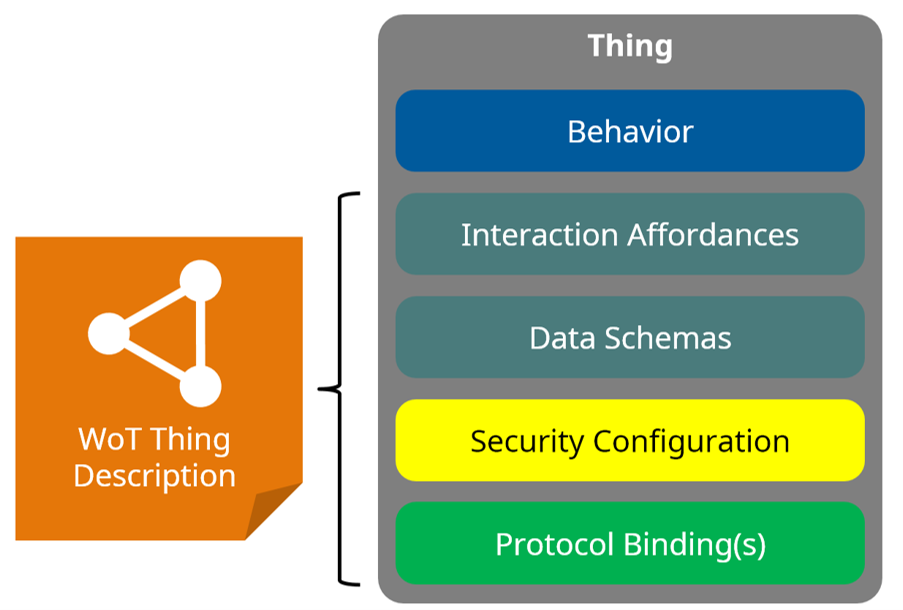
\includegraphics[width=0.3\textwidth]{Images/td.png}
    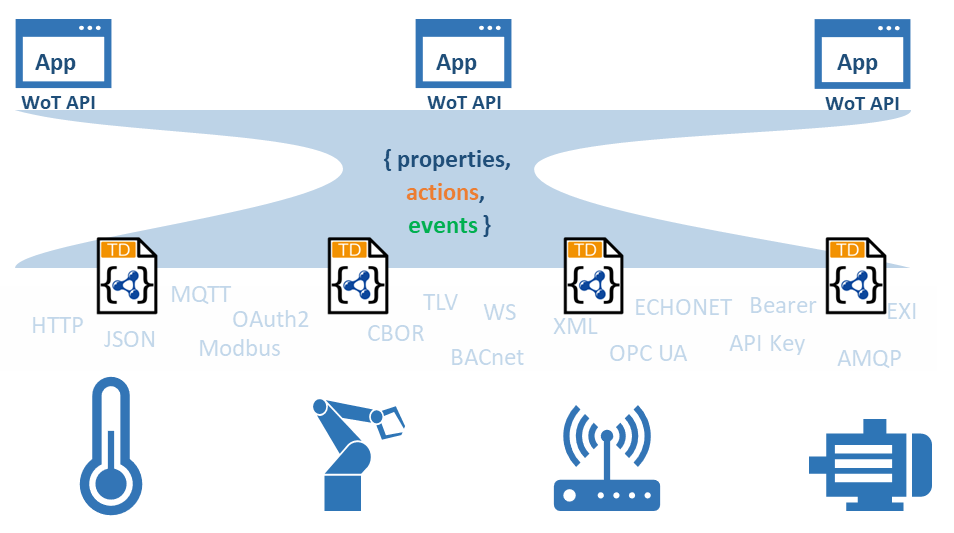
\includegraphics[width=0.35\textwidth]{Images/wot-mappings.png}
    \caption{\textbf{Table structure and entities} \\In general, WoT is a protocol agnostic approach and provides a common mechanism to define how specific protocols such as MQTT, HTTP, CoAP or Modbus can be mapped to the WoT's interaction properties-action-event abstraction.~\cite{W3CWOT2020}}
    \label{fig:image2}
\end{figure}



\textbf{CrateDB} is a distributed SQL database that combines the familiarity of relational queries with the scalability of NoSQL systems.  
It is particularly optimized for handling large volumes of \textbf{time-series data}.  

In this project, CrateDB was used to:
\begin{itemize}
    \item Store the \textbf{historical evolution} of dynamic entities, such as charging sessions and status changes,
    \item Enable efficient querying of attributes that evolve over time (e.g., \texttt{sessionStartTime}, \texttt{energyConsumed}, \texttt{sessionStatus}),
    \item Support analytical tasks and visualizations, since CrateDB integrates seamlessly with tools like Grafana.
\end{itemize}

Unlike MongoDB, which only keeps the latest state, CrateDB provided the \textbf{temporal dimension}, making it possible to analyze long-term patterns in charging behavior and infrastructure usage.

\subsection*{Complementarity}
Together, MongoDB and CrateDB formed a robust backend:
\begin{itemize}
    \item \textbf{MongoDB} ensured that the most up-to-date context was always available in real time,
    \item \textbf{CrateDB} provided scalability and analytical power for studying historical data.
\end{itemize}

This dual-database architecture guaranteed that the digital twin could support both \textbf{operational monitoring} and \textbf{strategic analysis}, which are equally important for the management of charging infrastructure.

\begin{table}[ht!]
    \centering
    \caption{Comparison of MongoDB and CrateDB in the backend architecture}
    \label{tab:mongodb-cratedb}
    \begin{tabular}{|p{3cm}|p{5cm}|p{5cm}|}
        \hline
        \textbf{Aspect} & \textbf{MongoDB} & \textbf{CrateDB} \\
        \hline
        Data model & Document-oriented (JSON-like) & Distributed SQL, optimized for time-series \\
        \hline
        Main role & Stores the \textbf{latest state} of NGSI-LD entities & Stores the \textbf{historical evolution} of dynamic entities \\
        \hline
        Strengths & Flexibility, schema-less design, fast context queries & Scalability, efficient time-series queries, integration with analytics tools \\
        \hline
        Typical usage & Querying current charging point or session status & Analyzing long-term charging behavior and energy consumption trends \\
        \hline
    \end{tabular}
\end{table}

\section{QuantumLeap and the Subscription Mechanism}

While MongoDB and CrateDB provide the persistence layer, the link between them is managed by \textbf{QuantumLeap (QL)}. 
QuantumLeap is a FIWARE component specifically designed for time-series management, enabling the storage and retrieval of temporal data associated with NGSI-LD entities.

\subsection*{Role of QuantumLeap}
QuantumLeap acts as middleware between the Orion Context Broker and CrateDB. Its main responsibilities include:
\begin{itemize}
    \item Receiving entity updates from Orion via the subscription mechanism,
    \item Transforming NGSI-LD payloads into a time-series format,
    \item Inserting temporal records into CrateDB for further analysis and visualization.
\end{itemize}

This ensures that the \textbf{current state} of entities is always maintained in MongoDB, while their \textbf{historical evolution} is stored in CrateDB.

\subsection*{The Subscription Mechanism}
At the core of QuantumLeap’s operation lies the \textbf{NGSI-LD subscription mechanism}.  
A subscription defines the conditions under which Orion notifies another component (in this case, QuantumLeap) about changes in entities.

A typical subscription includes:
\begin{itemize}
    \item \textbf{Target entity type:} e.g., \texttt{ChargingSession},
    \item \textbf{Attributes of interest:} e.g., \texttt{sessionStartTime}, \texttt{energyConsumed}, \texttt{sessionStatus},
    \item \textbf{Notification endpoint:} the URL of the QuantumLeap service,
    \item \textbf{Notification format:} NGSI-LD compliant JSON.
\end{itemize}

When an entity matching the subscription is created or updated, Orion automatically triggers a notification. QuantumLeap receives this message, processes it, and writes the corresponding time-series entry into CrateDB.

\subsection*{Practical Example}
In my project, I defined subscriptions for the \texttt{ChargingSession} entity. For each update (such as session initiation, charging progress, or completion), Orion sent a notification to QuantumLeap.  
As a result:
\begin{itemize}
    \item The current state of the session was updated in MongoDB,
    \item The full temporal history of the session was accumulated in CrateDB.
\end{itemize}

This mechanism ensured that the digital twin could support both \textbf{real-time monitoring} and \textbf{historical analysis} without additional manual intervention.

\subsection*{Summary}
By introducing QuantumLeap and the subscription mechanism, the backend architecture gained the ability to automatically capture time-series data.  
This allowed the digital twin to provide not only an instantaneous view of the charging infrastructure but also long-term insights into its operation, essential for analytics such as demand forecasting, anomaly detection, and infrastructure optimization.

\section{Data Visualization with Grafana}

To complete the backend pipeline, the digital twin framework integrates \textbf{Grafana} as the visualization layer.  
Grafana is an open-source analytics and monitoring platform that connects to CrateDB and provides interactive dashboards for exploring time-series data.

\subsection*{Role in the System}
While MongoDB and Orion Context Broker provide access to the current state of entities, and CrateDB stores their historical evolution, Grafana enables users to:
\begin{itemize}
    \item Visualize charging patterns over time (e.g., session durations, energy consumption curves),
    \item Compare usage between different charging stations or points,
    \item Monitor real-time infrastructure status alongside historical trends,
    \item Detect anomalies and inefficiencies through dashboards and alerts.
\end{itemize}

\subsection*{Practical Implementation}
In my project, I configured Grafana to connect directly to CrateDB as a data source.  
Using SQL queries, I extracted attributes from \texttt{ChargingSession} entities such as:
\begin{itemize}
    \item \texttt{sessionStartTime} and \texttt{sessionEndTime} for calculating durations,
    \item \texttt{energyConsumed} for analyzing charging demand,
    \item \texttt{sessionStatus} for monitoring operational states.
\end{itemize}

These values were then visualized through line charts, bar graphs, and time-series panels, providing an intuitive understanding of both short-term and long-term charging behavior.

\subsection*{Added Value}
Grafana dashboards not only improved the interpretability of the data but also:
\begin{itemize}
    \item Supported \textbf{decision-making}, by highlighting peak usage periods and energy demand fluctuations,
    \item Enhanced \textbf{operational monitoring}, by offering near real-time visualization of the infrastructure,
    \item Facilitated \textbf{communication}, as dashboards could be shared with stakeholders for reporting and strategic planning.
\end{itemize}

\subsection*{Summary}
By integrating Grafana with CrateDB, the digital twin achieved a complete data lifecycle: from \textbf{real-world collection} (E4C charging stations), to \textbf{standardized modeling} (NGSI-LD entities), to \textbf{backend persistence} (MongoDB + CrateDB), and finally to \textbf{human-centered visualization}.  
This closed the loop of the architecture, transforming raw data into actionable insights.

\section{Difficulties Encountered and Lessons Learned}

During the development of the digital twin system, several difficulties arose that influenced both the implementation process and the final design. These challenges can be grouped into three main areas: domain knowledge, technical resources, and deviations from the initial specifications.

\subsection*{Domain Knowledge and Data Modeling}
At the start of the project, my understanding of electric vehicle (EV) charging infrastructure was limited. This created challenges in defining appropriate entities and attributes for the NGSI-LD model.  
To overcome this, I conducted a thorough literature review and studied existing semantic models such as the \textbf{Brick ontology}. By combining insights from academic papers with standardized data models, I was able to enrich my understanding and build a more consistent representation of charging infrastructure.

\subsection*{Limited Documentation on FIWARE}
Another challenge was the lack of up-to-date resources for FIWARE components. Many official tutorials had not been maintained for several years, which made it difficult to find reliable references.  
For example:
\begin{itemize}
    \item Initially, I planned to use \textbf{WireCloud} as the front-end visualization tool, but discovered that it had not been actively maintained for nearly eight years. This forced me to abandon the idea and search for more sustainable alternatives such as Grafana.
    \item For time-series data persistence, I first experimented with \textbf{Mintaka}, but found that its capabilities were limited compared to QuantumLeap. Consequently, I decided to replace Mintaka with QuantumLeap.
\end{itemize}

\subsection*{Integration Challenges with NGSI-LD}
QuantumLeap was originally designed with native support for NGSI-v2 rather than NGSI-LD, which introduced compatibility issues. Through detailed analysis of the official documentation and extensive testing, I was able to configure and adapt QuantumLeap for NGSI-LD entities.  
This process required additional research and debugging but ultimately strengthened my understanding of the FIWARE ecosystem and its evolution.

\subsection*{Differences from Initial Specifications}
Compared to the initial plan, several significant changes were made:
\begin{itemize}
    \item WireCloud was excluded due to lack of maintenance, and Grafana was adopted instead for visualization.
    \item Mintaka was replaced by QuantumLeap for improved time-series persistence.
    \item Adjustments were necessary to ensure full NGSI-LD compliance, particularly when integrating QuantumLeap.
\end{itemize}

\subsection*{Summary}
Although these difficulties introduced delays and required adaptations, they also offered valuable learning opportunities. I gained deeper knowledge of EV charging infrastructures, developed skills in semantic data modeling, and built resilience in navigating incomplete or outdated documentation. Ultimately, the adjustments strengthened the robustness and sustainability of the final system design.



% \section{Listes et tableaux}

% \textbf{Insérer une liste~:}
% \begin{itemize}
%     \item Premier niveau
%     \begin{itemize}
%         \item[(i)] Deuxième niveau
%         \item[(ii)] Un autre élément au deuxième niveau
%     \end{itemize}
%     \item Un autre élément au premier niveau
%         \begin{itemize}
%         \item[(a)] Deuxième niveau
%         \item[(b)] Un autre élément au deuxième niveau
%     \end{itemize}
% \end{itemize}
% \bigskip

% \textbf{Insérer un tableau simple~:} 
% \begin{table}[H]
%     \centering
%     \begin{tabular}{|c|c|c|c|c|c|c|c|c|c|}
%         \hline
%         A & B & C & D & E & F & G & H & I & \dots \\
%         \hline
%         1 & 2 & 3 & 4 & 5 & 6 & 7 & 8 & 9 & \dots\\
%         10 & 11 & 12 & 13 & 14 & 15 & 16 & 17 & 18 & \dots \\
%         \hline
%     \end{tabular}
%     \caption{\textbf{Titre.} \lipsum[1][1-3]}
%     \label{tab:table-label}
% \end{table}

% \textbf{Autre style de tableau~:} 
% \begin{table}[H]
%     \centering
%     \begin{tabular}{c c c c c}
%         \hline
%         \textbf{Col1} & \textbf{Col2} & \textbf{Col3} & \textbf{Col4} & \textbf{Col5} \\
%         \hline
%         1 & 2 & 3 & 4 & 5 \\
%         1 & 2 & 3 & 4 & 5 \\
%         \hline
%     \end{tabular}
%     \caption{\textbf{Titre.} \lipsum[1][1-3]}
%     \label{tab:table-label}
% \end{table}


% \section{Insertion de code Python}
% \textbf{Insérer du code en \textit{inline}~:} \texttt{print("Hello, World!")}.\\


% \textbf{Insérer du code en \textit{inline} avec coloration syntaxique~:} \mintinline{python}{print("Hello, World!")}.\\

% \textbf{Insérer du code en bloc avec coloration syntaxique~:} 
% \begin{minted}[bgcolor=codebg,fontsize=\small,frame=lines,linenos]{python}
%     "@context": {
%         "type": "@type",
%         "id": "@id",
%         "ngsi-ld": "https://uri.etsi.org/ngsi-ld/",
%         "fiware": "https://uri.fiware.org/ns/data-models#",
%         "schema": "https://schema.org/",
%         "ChargingPoint": "fiware:ChargingPoint",
%         "ChargingPointStatus": "fiware:ChargingPointStatus",
%         "ChargingSession": "fiware:ChargingSession",
%         "ChargingStation": "fiware:ChargingStation"}
% \end{minted}



% \section{Expressions mathématiques}
% \subsection{Théorèmes, propositions, définitions, lemmes, demonstrations...}

% \begin{theorem}
%     \lipsum[1][1-4]
% \end{theorem}

% \begin{proof}
%     \lipsum[1][1-4]
% \end{proof}

% \begin{proposition}
%     \lipsum[1][1-4]
% \end{proposition}

% \begin{definition}
%     \lipsum[1][1-4]
% \end{definition}

% \begin{remark}
%     \lipsum[1][1-4]
% \end{remark}

% \begin{lemma}
%     \lipsum[1][1-4]
% \end{lemma}


% \subsection{Equations et calculs sur plusieurs lignes}

% \subsubsection*{Une simple équation}
% \begin{equation}
%     e = mc^2
% \end{equation}

% \subsubsection*{Une équation sur plusieurs lignes}
% \begin{equation}
%     \begin{split}
%         \mathbb{E}(aX + Y) &= \mathbb{E}(aX) + Y\\
%                            &= a\mathbb{E}(X) + Y
%     \end{split}
% \end{equation}

% \subsubsection*{Une équation avec plusieurs cas}
% \begin{equation}
%     u_n =
%     \begin{cases}
%         1 \text{ if } n\equiv0 \mod 2\\
%         0 \text{ if } n\equiv1 \mod 2 \\
%     \end{cases}
% \end{equation}

% \subsubsection*{Insérer une série de calculs}
% \begin{align*}
%     x &= 0.999\ldots \\
%     10x &= 9.999\ldots \\
%     10x - x &= 9.999\ldots - 0.999\ldots \\
%     9x &= 9 \\
%     x &= 1 \\
%     0.999\ldots &= 1
% \end{align*}

% \subsection{Utilisation du glossaire}

% \newglossaryentry{esperance}{
%     name=espérance,
%     description={Valeur moyenne théorique d'une variable aléatoire}
% }


% Référence au glossaire : \gls{esperance}.  




